% !TEX root = /home/frank/School/thesis_text/thesis.tex

\chapter{Performance Analysis}

\section{Pragma's influencing the memory architecture implementation}

The way memory accesses are implemented are an important factor influencing the performance of an IP-Core. Buffers have a large influence on the operational intensity. Increasing operational intensity moves the implementation from memory bound area of the roofline model to the compute bound area of the roofline model.\\
In \emph{High Level} programming languages memory gets abstracted to variables and array's. These abstractions need to be translated into something that can be implemented in hardware. For FPGA's this means choosing between \emph{block ram} or registers. The process of translating the memory constructs into the most fitting type of physical memory is controlled by the HLS compiler but can be influenced by using directives or pragma's. Especially the way arrays are translated into hardware is of importance. For this purpose a couple of directives are available.\\

\begin{description}

\item[Resource] lets the programmer determine which component will be used to map a certain array to.

\item[Array\_Map] Maps several smaller arrays to the same memory to decrease the resource consumption.

\item[Array\_Partition] Determines how a certain array will be partitioned into smaller arrays each using their own memory to avoid the bottleneck of having to perform multiple consecutive reads. This directive also allows to partition an array completely into registers.

\item[Array\_Reshape] Will rearrange an array so the elements have a larger word width. This improves the performance of the memory while maintaining the same resource consumption.

\end{description}

In systems doing video processing buffers are usually employed to exploit the spatial and temporal data locality. In the example of the TRD there are 2 abstractions implemented: \texttt{ap\_linebuffer} and \texttt{ap\_window}.

\subsection{\texttt{ap\_linebuffer} Class}

The class \texttt{ap\_linebuffer} is a generic C++ implementation of the linebuffer described in XAPP793. A linebuffer is described as a multi-dimensional shift-register. A linebuffer needs to be able to be read and written to in the same cycle to maximize performance. The dual port nature of block RAM makes it the ideal component for this abstraction.
Because the \texttt{ap\_linebuffer} class is generic its behavior needs to be defined in the application. The template for the \texttt{ap\_linebuffer} class is \texttt{<typename T, int LROW, int LCOL>}. A type, the number of rows and the number of columns need to be specified. This is done in the \texttt{sobel.h} file by the following line:

\begin{verbatim}
typedef ap_linebuffer<unsigned char, 3, MAX_WIDTH> Y_BUFFER;
\end{verbatim}

The parameters of the template are used to determine the size of the only variable of the class, -the array M of type T with LROW rows and LCOL columns.\\
This array get partitioned by the following directive:

\begin{verbatim}
#pragma AP ARRAY_PARTITION variable=M dim=1 complete
\end{verbatim}

This means that the first dimension, the number of rows, get partitioned into different block RAMs. This is also reported by the vivado HLS tool. buff\_A is the line buffer used throughout the implementation.\\

\medskip

\begin{figure}[h]
\centering
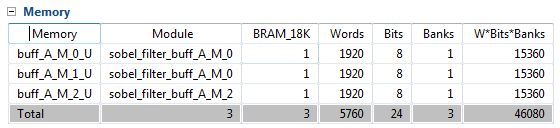
\includegraphics[scale=0.8]{/home/frank/School/thesis_text/images/trd_original_buffer_partitioning.PNG} 
\caption{paritioning of an array in multiple block RAM instances}
\end{figure}


\subsection{\texttt{ap\_window} Class}

The second class used in the application is a generic implementation of the memory window described in XAPP793. It is a combination of shift-registers forming a 2-dimensional data storage element of N pixels centered on a pixel P. Usually these are implemented as flip-flops because they contain relatively few elements who need to be simultaneously available for a calculation. This is achieved through completely partitioning the memory into registers, preventing it from being implemented by a block RAM.
The template of \texttt{ap\_window} is \texttt{<typename T, int LROW, int LCOL>}. These parameters are used for the only variable in the class, an array M of type T with LROW rows and LCOL cols. Analog to the linebuffer class the programmer here also needs to define the type, number of rows and number of columns of array M. The array gets paritioned into registers by the following directive:

\begin{verbatim}
#pragma AP ARRAY_PARTITION variable=M dim=0 complete
\end{verbatim}

The \texttt{dim=0} means that all dimensions should be partitioned. The \texttt{complete} keyword signifies that this partitioning should be done for the whole array.


\subsection{influence of memory architecture on the operational intensity}

This hierarchical structure of the memory influences the operational intensity of the algorithm. The numerator is determined by the number of bytes being processed by the core. Every iteration one value gets read from the external memory and one value gets written.  There are 32 bits per pixel, so there are 4 bytes per pixel. this means that with height H and width W there are:

\[
4 * 2 * ( H * W )
\]

bytes being read/written to/from the memory. This is the denominator in the expression of the operational intensity.\\
The numerator is dependent on the number of pixels being calculated by the core. The core used in the TRD doesn't calculate the pixels on the outer rim of the image and instead uses these as padding. 

\begin{lstlisting}

if( row <= 1 || col <= 1 || row > (rows-1) || col > (cols-1)){
		
		edge.R = edge.G = edge.B = 0;
		
}
//Sobel operation on the inner portion of the image
else{

		edge = sobel_operator( ... );
		
}		
\end{lstlisting}

This branching needs to be taken into consideration for the expression of the computational intensity. The expression for the numerator is given by:

\[
( H * W ) -[ ( 4 * W ) + 4 * ( H - 4 )]
\]


the complete expression is then given by:

\[
\frac{( H * W ) -[ ( 4 * W ) + 4 * ( H - 4 )]}{4 * 2 * ( H * W )}
\]








\section{Pramga's influencing throughput}

\subsection{Original TRD}

The original TRD has 3 pragma's applied to it:

\begin{scriptsize}
\begin{verbatim}
set_directive_loop_flatten -off "sobel_filter/sobel_filter_label0"
set_directive_dependence -variable &buff_A -type inter -dependent false "sobel_filter/sobel_filter_label0"
set_directive_pipeline -II 1 "sobel_filter/sobel_filter_label0"
\end{verbatim}
\end{scriptsize}

These all influence the system in a distinct way.

\paragraph{Loop Flattening} This directive combines nested loops. This removes the need for the clockcycle needed to enter and leave the loop. It needs to be applied to the inner loop of a set of nested loops. In the TRD loop flattening is explicitly disabled.

\paragraph{Dependence} The compiler tries to identify dependencies between calculations or resources. Sometimes this automatic identification of dependencies is too conservative because the compiler doesn't have some information. For this reason the \emph{dependence} directive exists, allowing the programmer to explicitly state that there are or aren't dependencies for a certain variable. There are two types of dependence:

\begin{description}
\item[Inter] The dependence is between different iterations of the same loop. If the dependence is set to false this will allow the loop to be unrolled
\item[Intra] The dependence is inside the iteration. If the dependence is set to be false the compiler will attempt to reorder the operations for the most optimal performance.
\end{description}

In the case of the TRD the inter-dependence of the variable buff\_A is set to false.

\paragraph{Pipeline} The directive set\_directive\_pipeline is used to control the pipelining of loops and functions. Each function or loop on which this directive is used can read a new input every N clockcycles. This variable N is called the \emph{Initiation Interval} or II for short. In the case of the TRD pipelining is applied to the inner loop, with an Initiation Interval equal to 0.


\subsubsection{Throughput}
\label{sec:original_througput}

Given the analysis generated by Vivado HLS presented in table \ref{tab:analysis_data} it is possible to calculate the throughput of the system. First of all it needs to be noted whether the system satisfies the timing requirements. The analysis gives us an estimated clock period of 4.2 ns with an uncertainty of 0.62 ns placing it well within the bounds of the required 5 ns clock period.
The system needs 22 cycles to complete. Of these, there are 2 initialization cycles, 20 cycles to finish the outer loop, of which 19 cycles are the inner loop. The system employs pipelining on the innermost loop, which results in an initiation interval of 1.

N is the number of cycles necessary to calculate one frame:


\[
N =  \text{init cycles} + \text{outer loop iterations} * ( \text{iteration cycles} + \text{inner loop iterations} - 1)
\]


These cycles all take a certain time to complete:

\[
total\ time = N * cycle\ time
\]

The number of frames per second is then given by:

\[
FPS = \frac{1}{total\ time}
\]

Entering the numbers found in table \ref{table:HLS_analysis} gives us a value of 95.37 frames per second. Given that HDMI has a 60 Hz refresh rate this system satisfies that constraint.


\subsection{No pragma's}

The original system performance satisfies the real time constraint placed on the system. To study the impact the directives have on the performance of the system all directives were removed from the  system. The analysis generated by Vivado HLS is presented in the second column of table \ref{table:HLS_analysis}. The first observation that can be done is that the system performs the same operation in only 16 clock cycles instead of 22, a decrease of 27\%. Because the system has no pipelining the initiation interval is 14 cycles. A new value gets read each iteration.

The number of cycles needed to calculate one frame is given by:

\[
N = init\ cycles + outer\ loop\ iterations * (inner\ loop\ iterations * inner\ loop\ cycles) 
\]


Knowing the number of cycles the throughput can be calculated the same way it is done in section \ref{sec:original_througput}. This gives us a value of 0.47 frames per second, a 203 times decrease in performance.

\subsection{Loop flatten on}

The next effect that can be studies is the effect of turning loop flattening on. This is done with the following directives:

\begin{scriptsize}
\begin{verbatim}
set_directive_dependence -variable &buff_A -type inter -dependent false "sobel_filter/sobel_filter_label0"
set_directive_pipeline -II 1 "sobel_filter/sobel_filter_label0"
set_directive_loop_flatten "sobel_filter/sobel_filter_label0"
\end{verbatim}
\end{scriptsize}

\subsection{Loop flattening with Initiation Interval 2}




% Table specifying the resource consumption of the different solutions

\begin{table}[H]
\begin{center}
\begin{tabular}{rcccc}
\toprule
 & \textbf{BRAM\_18K} & \textbf{DSP48E} & \textbf{FF} & \textbf{LUT}\\ \midrule
\textbf{Original directives} & 3 & 23 & 1487 & 1412 \\ 
\textbf{No pragma} & 5 & 4 & 802 & 1475 \\ 
\textbf{loop\_flatten\_on} & 3 & 23 & 1764 & 1668 \\ 
\textbf{loop\_flatten\_II\_2} & 3 & 23 & 1777 & 1875 \\ 
\textbf{no\_dependence} & 3 & 19 & 1487 & 1412 \\ 
\textbf{no\_pipeline} & 5 & 4 & 802 & 1475 \\ 
\textbf{only dependence} & 5 & 4 & 786 & 1534 \\ 
\textbf{only loop flattening} & 5 & 8 & 1050 & 1783 \\ 
\textbf{only pipelining} & 3 & 23 & 1851 & 1849 \\ \bottomrule
\end{tabular}
\end{center}
\caption{Utilization Estimates}
\label{tab:utilization_estimates}
\end{table}



\begin{landscape}

\begin{table}[htbp]
\begin{center}

	\begin{tabular}{rccccc}
	\toprule
	 & \textbf{Original directives} & \textbf{No pragma} & \textbf{loop\_flatten\_on} & \textbf{loop\_flatten\_II\_2} & \textbf{no\_dependence} \\ \midrule
	
	\textbf{Estimated Clock (ns)} & 4,2 & 4,35 & 5,25 & 4,2 & 4,2 \\ 
	\textbf{Uncertainty (ns)} & 0,62 & 0,62 & 0,62 & 0,62 & 0,62 \\ 
	\textbf{cycle time (ns)} & 5 & 5 & 5,25 & 5 & 5 \\ 
	\textbf{total cycles} & 22 & 16 & 28 & 29 & 23 \\ 
	\textbf{init} & 2 & 2 & 8 & 8 & 2 \\ 
	\textbf{outer loop} & 20 & 14 & 20 & 21 & 21 \\ 
	\textbf{inner loop} & 19 & 13 & N/A & N/A & 20 \\ 
	\textbf{pipelining outer} & no & no & yes & yes & no \\ 
	\textbf{pipelining inner} & yes & no & N/A & N/A & yes \\ 
	\textbf{Initiation Interval} & 1 & 14 & 1 & 2 & 1 \\ \bottomrule
	\end{tabular}

	\bigskip

	\begin{tabular}{rccccc}
	\toprule
	 & \textbf{no\_pipeline} & \textbf{only dependence} & \textbf{only loop flattening} & \textbf{only pipelining} & \textbf{only pipelining II 2} \\ \midrule
	\textbf{Estimated Clock (ns)} & 4,35 & 4,35 & 4,35 & 4,2 & 4,2 \\ 
	\textbf{Uncertainty (ns)} & 0,62 & 0,62 & 0,62 & 0,62 & 0,62 \\ 
	\textbf{cycle time (ns)} & 5 & 5 & 5 & 5 & 5 \\ 
	\textbf{total cycles} & 17 & 16 & 22 & 31 & 31 \\ 
	\textbf{init} & 2 & 2 & 8 & 8 & 8 \\ 
	\textbf{outer loop} & 15 & 14 & 14 & 23 & 23 \\ 
	\textbf{inner loop} & 14 & 13 & N/A & N/A & N/A \\ 
	\textbf{pipelining outer} & no & no & no & yes & yes \\ 
	\textbf{pipelining inner} & no & no & no & no & no \\ 
	\textbf{Initiation Interval} & 15 & 14 & 14 & 2 & 2 \\ \bottomrule
	\end{tabular}


\end{center}
\caption{Analysis Data}
\label{tab:analysis_data}
\end{table}
\end{landscape}

% \begin{landscape}
% \begin{table}[htbp]
% \begin{center}
% \begin{tabular}{|r|r|r|r|r|r|}
% \hline
%  & \textbf{no\_pipeline} & \textbf{only dependence} & \textbf{only loop flattening} & \textbf{only pipelining} & \textbf{only pipelining II 2} \\ \hline
%  &  &  &  &  &  \\ \hline
% \textbf{Estimated Clock (ns)} & 4,35 & 4,35 & 4,35 & 4,2 & 4,2 \\ \hline
% \textbf{Uncertainty (ns)} & 0,62 & 0,62 & 0,62 & 0,62 & 0,62 \\ \hline
% \textbf{cycle time (ns)} & 5 & 5 & 5 & 5 & 5 \\ \hline
% \textbf{total cycles} & 17 & 16 & 22 & 31 & 31 \\ \hline
% \textbf{init} & 2 & 2 & 8 & 8 & 8 \\ \hline
% \textbf{outer loop} & 15 & 14 & 14 & 23 & 23 \\ \hline
% \textbf{inner loop} & 14 & 13 & N/A & N/A & N/A \\ \hline
% \textbf{pipelining outer} & no & no & no & yes & yes \\ \hline
% \textbf{pipelining inner} & no & no & no & no & no \\ \hline
% \textbf{Initiation Interval} & 15 & 14 & 14 & 2 & 2 \\ \hline
% \end{tabular}
% \end{center}
% \caption{Analysis Data Continued}
% \label{tab:analysis_data_cont}
% \end{table}
% \end{landscape}



